\documentclass[border=10pt]{standalone}

\usepackage{tikz}
\usepackage{tikzsymbols}
\usetikzlibrary{calc,patterns,shapes.geometric}

\def\centerarc[#1](#2)(#3:#4:#5){\draw[#1] ($(#2)+({#5*cos(#3)},{#5*sin(#3)})$) arc (#3:#4:#5);}

\begin{document}
	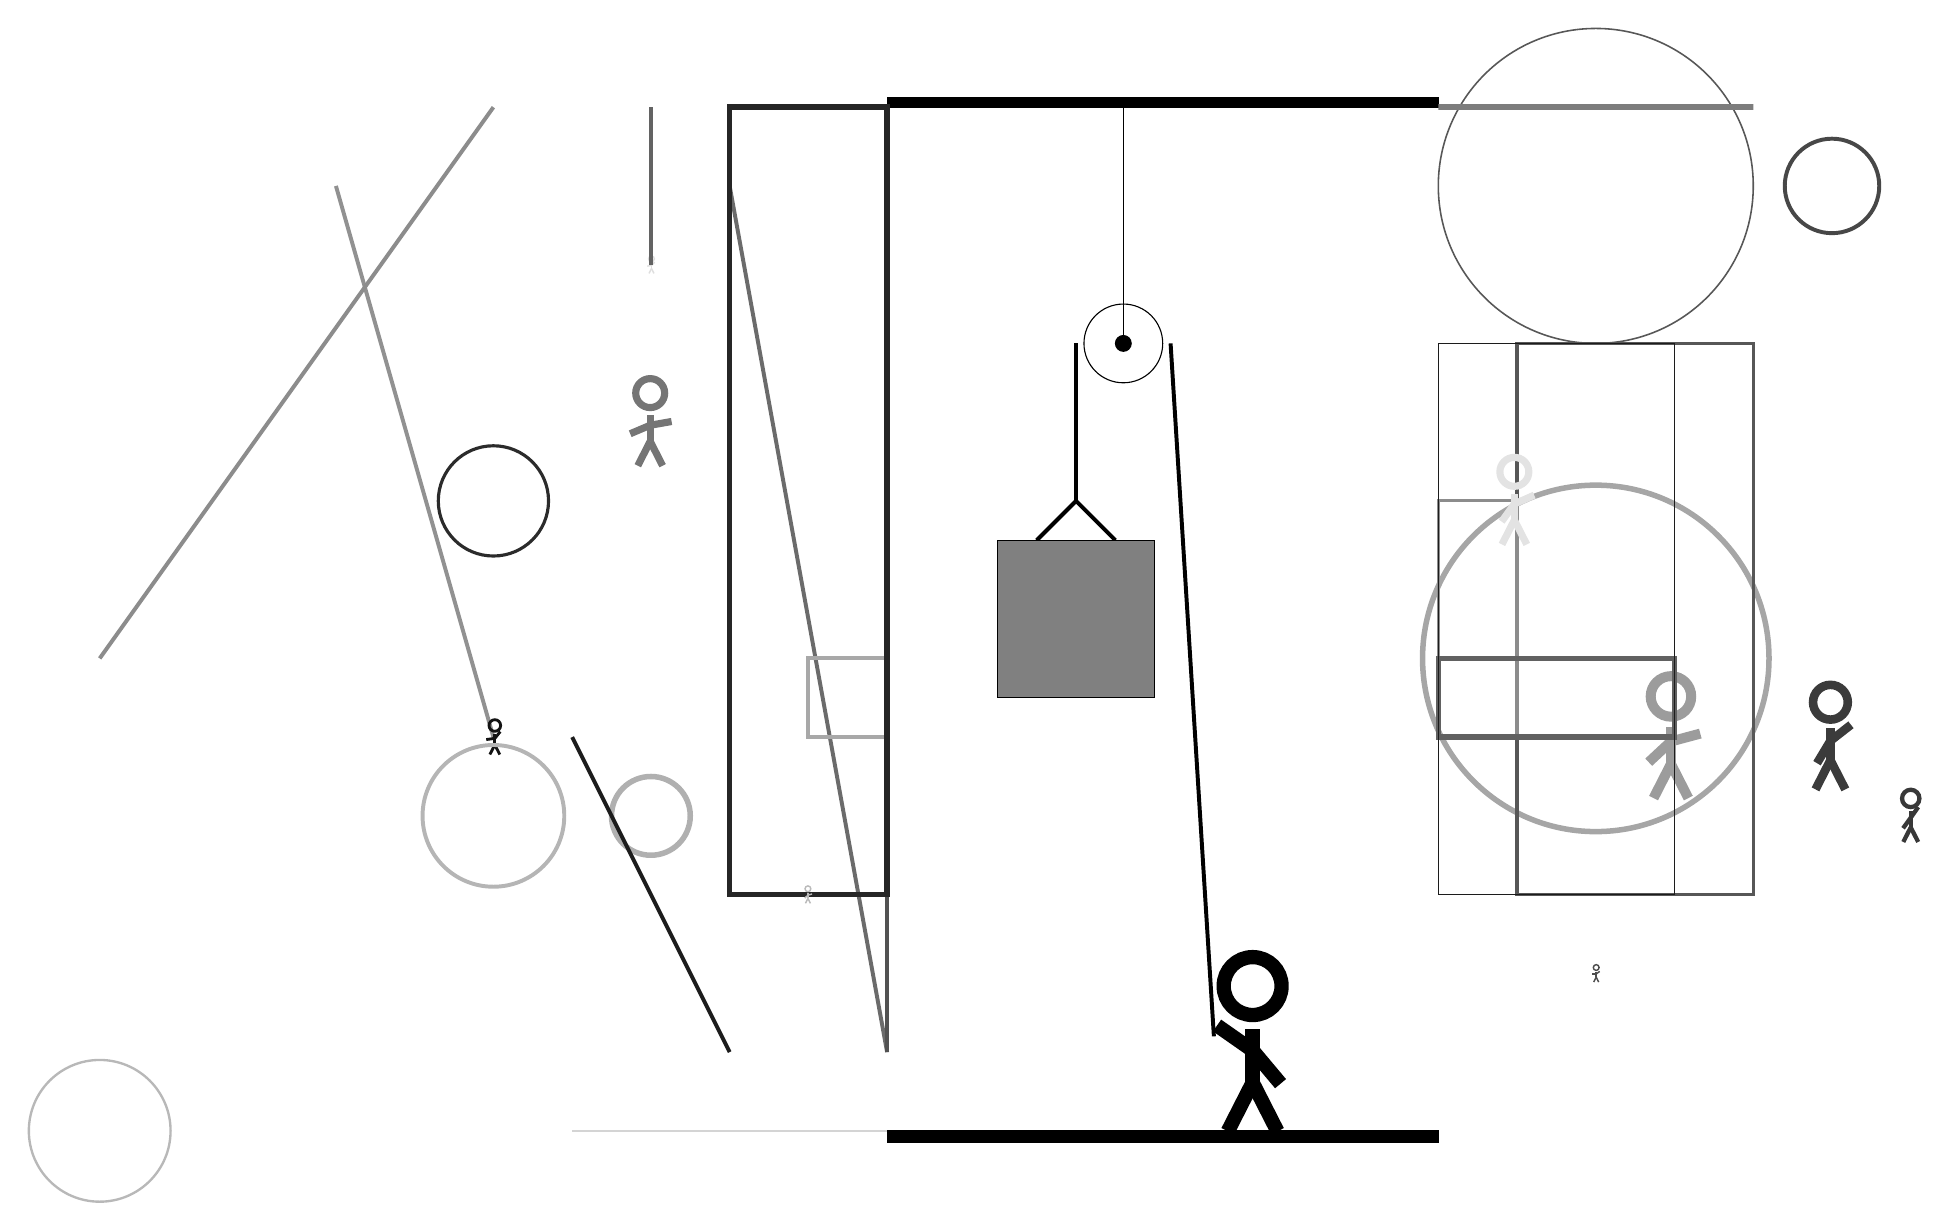
\begin{tikzpicture}
		%%%%% START %%%%%
		
		\draw[fill=black] (-2, 10) rectangle (5, 10.125);
		
		\draw (1, 7) circle (0.5);
		\draw[fill=black] (1, 7) circle (0.1);
		\draw (1, 10) -- (1, 7);
		
		\draw[line width=0.5mm] (-0.1, 4.5) -- (0.4, 5.0) -- (0.9, 4.5);
		\draw[fill=black!50] (-0.6, 4.5) rectangle (1.4, 2.5);
		
		\node[line width=0.7mm, color=black!13] at (-5, 8) {\Strichmaxerl[1][12][45]};
		
		\node[line width=0.6mm, color=black!39] at (8, 2) {\Strichmaxerl[7][43][15]};
		\draw [line width=0.7mm, color=black!31](-5, 1) circle (0.5);
		\draw [line width=0.7mm, color=black!35](7, 3) circle (2.2);
		\draw[line width=0.5mm, color=black!58](-2, -2) -- (-4, 9);
		\draw[line width=0.5mm, color=black!68] (-2, 7) rectangle (-2, -2);
		\node[line width=0.7mm, color=black!54] at (-5, 6) {\Strichmaxerl[5][23][10]};
		\draw [line width=0.4mm, color=black!83](-7, 5) circle (0.7);
		\node[line width=0.3mm, color=black!78] at (11, 1) {\Strichmaxerl[3][54][55]};
		\draw[line width=0.5mm, color=black!89](-6, 2) -- (-4, -2);
		
		\draw[line width=0.5mm, color=black!34] (-2, 3) rectangle (-3, 2);
		
		\draw[line width=0.4mm, color=black!66] (6, 7) rectangle (9, 0);
		\draw[line width=0.5mm, color=black!43](-7, 2) -- (-9, 9);
		\draw[line width=0.4mm, color=black!45] (5, 5) rectangle (6, 2);
		\draw[line width=0.5mm, color=black!45](-7, 10) -- (-12, 3);
		\draw [line width=0.3mm, color=black!28](-12, -3) circle (0.9);
		\draw [line width=0.2mm, color=black!66](7, 9) circle (2.0);
		\draw[line width=0.5mm, color=black!61](-5, 10) -- (-5, 8);
		\draw [line width=0.5mm, color=black!72](10, 9) circle (0.6);
		\draw[line width=0.7mm, color=black!85] (-4, 0) rectangle (-2, 10);
		\node[line width=0.3mm, color=black!93] at (-7, 2) {\Strichmaxerl[2][8][51]};
		\node[line width=0.6mm, color=black!77] at (10, 2) {\Strichmaxerl[6][59][38]};
		\draw [line width=0.5mm, color=black!29](-7, 1) circle (0.9);
		\draw[line width=0.7mm, color=black!62] (5, 2) rectangle (8, 3);
		\draw[line width=0.7mm, color=black!51] (5, 10) rectangle (9, 10);
		\node[line width=0.7mm, color=black!27] at (-3, 0) {\Strichmaxerl[1][42][17]};
		\node[line width=0.4mm, color=black!70] at (7, -1) {\Strichmaxerl[1][0][36]};
		\node[line width=0.2mm, color=black!11] at (6, 5) {\Strichmaxerl[5][54][24]};
		
		\draw[line width=0.3mm, color=black!17] (-2, -3) rectangle (-6, -3);
		\draw[line width=0.2mm, color=black!89] (5, 7) rectangle (8, 0);
		
		\draw[line width=0.5mm] (0.4, 7) -- (0.4, 5.0);
		\centerarc[line width=0.5mm](1, 7)(0:180:0.6);
		\draw[line width=0.5mm](1.6, 7) -- (2.15, -1.8);
		
		\node at (2.6, -1.9) {\Strichmaxerl[10][-35][-50]};
		
		\draw[fill=black] (-2, -3) rectangle (5, -3.15);
		
		%%%%% END %%%%%
	\end{tikzpicture}
\end{document}